% !TEX spellcheck = en_US
% !TEX spellcheck = LaTeX

\documentclass[letterpaper,english,10pt]{article}

\usepackage{%
	amsfonts,%
	amsmath,%	
	amssymb,%
	amsthm,%
	babel,%
	bbm,%
	%biblatex,%
	caption,%
	centernot,%
	color,%
	enumerate,%
	%enumitem,%
	epsfig,%
	epstopdf,%
	etex,%
	fancybox,%
	framed,%
	fullpage,%
	%geometry,%
	graphicx,%
	hyperref,%
	latexsym,%
	mathptmx,%
	mathtools,%
	multicol,%
	pgf,%
	pgfplots,%
	pgfplotstable,%
	pgfpages,%
	proof,%
	psfrag,%
	%subfigure,%	
	tikz,%
	times,%
	ulem,%
	url,%
	xcolor,%
	mathpazo
}

\definecolor{shadecolor}{gray}{.95}%{rgb}{1,0,0}
\usepackage[margin=1in,top=0.75in]{geometry}
\usepackage[mathscr]{eucal}
\usepgflibrary{shapes}
\usepgfplotslibrary{fillbetween}
\usetikzlibrary{%
  arrows,%
  backgrounds,%
  chains,%
  decorations.pathmorphing,% /pgf/decoration/random steps | erste Graphik
  decorations.text,% 
  matrix,%
  positioning,% wg. " of "
  fit,%
  patterns,%
  petri,%
  plotmarks,%
  scopes,%
  shadows,%
  shapes.misc,% wg. rounded rectangle
  shapes.arrows,%
  shapes.callouts,%
  shapes%
}

%\pgfplotsset{compat=newest} %<------ Here
\pgfplotsset{compat=1.11} %<------ Or use this one

\theoremstyle{plain}
\newtheorem{thm}{Theorem}[section]
\newtheorem{lem}[thm]{Lemma}
\newtheorem{prop}[thm]{Proposition}
\newtheorem{cor}[thm]{Corollary}
\newtheorem{clm}[thm]{Claim}

\theoremstyle{definition}
\newtheorem{axiom}[thm]{Axiom}
\newtheorem{defn}[thm]{Definition}
\newtheorem{conj}[thm]{Conjecture}
\newtheorem{exmp}[thm]{Example}
\newtheorem{exerc}[thm]{Exercise}
\newtheorem{assum}[thm]{Assumptions}

\theoremstyle{remark}
\newtheorem{rem}[thm]{Remark}
\newtheorem{note}[thm]{Note}

\newcommand{\Cov}{\operatorname{Cov}}
%\newcommand{\det}{\operatorname{det}}
\newcommand{\Real}{\mathbb{R}}
\newcommand{\tr}{\operatorname{tr}}
%\newcommand{\Var}{\operatorname{Var}}

\DeclareMathOperator{\sign}{sign}
%\renewcommand{\proof}[1]{\begin{proof}#1\end{proof}}
\newcommand{\EQ}[1]{\begin{equation*}#1\end{equation*}}
\newcommand{\EQN}[1]{\begin{equation}#1\end{equation}}
\newcommand{\eq}[1]{\begin{align*}#1\end{align*}}
\newcommand{\meq}[2]{\begin{xalignat*}{#1}#2\end{xalignat*}}
\newcommand{\norm}[1]{\left\lVert#1\right\rVert}
\newcommand{\abs}[1]{\left\lvert#1\right\rvert}
\newcommand{\expect}[1]{\mathbb{E}\left[{#1}\right]}
\newcommand{\prob}[1]{\mathbb{P}\left[{#1}\right]}
\newcommand{\given}{\; \big\vert \;} 
\newcommand{\set}[1]{\left\{#1\right\}} 
\newcommand{\indicator}[1]{\mathbb{1}_{\set{#1}}} 
\newcommand{\inner}[1]{\left\langle#1\right\rangle}
\newcommand{\red}[1]{\textcolor{red}{#1}} 
\newcommand{\E}[1]{\mathbb{E}\left[#1\right]}
\newcommand{\Var}[1]{\operatorname{Var}\left[#1\right]}

\newcommand{\D}{\mathbb{D}}
%\newcommand{\E}{\mathbb{E}}
\newcommand{\N}{\mathbb{N}}
\renewcommand{\P}{\mathbb{P}}
\newcommand{\Q}{\mathbb{Q}}
\newcommand{\R}{\mathbb{R}}
\newcommand{\Z}{\mathbb{Z}}

\newcommand{\bU}{\mathbf{1}}
\newcommand{\bx}{\mathbf{x}}

\newcommand{\cB}{\mathcal{B}}
\newcommand{\cC}{\mathcal{C}}
\newcommand{\cD}{\mathcal{D}}
\newcommand{\cF}{\mathcal{F}}
\newcommand{\cG}{\mathcal{G}}
\newcommand{\cH}{\mathcal{H}}
\newcommand{\cO}{\mathcal{O}}
\newcommand{\cT}{\mathcal{T}}
\newcommand{\cX}{\mathcal{X}}
\newcommand{\cY}{\mathcal{Y}}

\newcommand{\sA}{\mathscr{A}}
\newcommand{\sB}{\mathscr{B}}
\newcommand{\sC}{\mathscr{C}}
\newcommand{\sD}{\mathscr{D}}
\newcommand{\sE}{\mathscr{E}}
\newcommand{\sF}{\mathscr{F}}
\newcommand{\sG}{\mathscr{G}}
\newcommand{\sH}{\mathscr{H}}
\newcommand{\sL}{\mathscr{L}}
\newcommand{\dO}{\mathscr{O}}
\newcommand{\sS}{\mathscr{S}}
\newcommand{\sT}{\mathscr{T}}
\newcommand{\sX}{\mathscr{X}}
\newcommand{\sY}{\mathscr{Y}}
\newcommand{\sZ}{\mathscr{Z}}

% Debug
\newcommand{\todo}[1]{\begin{color}{blue}{{\bf~[TODO:~#1]}}\end{color}}

% a few handy macros

\renewcommand{\le}{\leqslant}
\renewcommand{\ge}{\geqslant}
\newcommand\matlab{{\sc matlab}}
\newcommand{\goto}{\rightarrow}
\newcommand{\bigo}{{\mathcal O}}
%\newcommand{\half}{\frac{1}{2}}
%\newcommand\implies{\quad\Longrightarrow\quad}
\newcommand\reals{{{\rm l} \kern -.15em {\rm R} }}
\newcommand\complex{{\raisebox{.043ex}{\rule{0.07em}{1.56ex}} \hskip -.35em {\rm C}}}


% macros for matrices/vectors:

% matrix environment for vectors or matrices where elements are centered
\newenvironment{mat}{\left[\begin{array}{ccccccccccccccc}}{\end{array}\right]}
\newcommand\bcm{\begin{mat}}
\newcommand\ecm{\end{mat}}

% matrix environment for vectors or matrices where elements are right justifvied
\newenvironment{rmat}{\left[\begin{array}{rrrrrrrrrrrrr}}{\end{array}\right]}
\newcommand\brm{\begin{rmat}}
\newcommand\erm{\end{rmat}}

% for left brace and a set of choices
%\newenvironment{choices}{\left\{ \begin{array}{ll}}{\end{array}\right.}
\newcommand\when{&\text{if~}}
\newcommand\otherwise{&\text{otherwise}}
% sample usage:
%  \delta_{ij} = \begin{choices} 1 \when i=j, \\ 0 \otherwise \end{choices}


% for labeling and referencing equations:
\newcommand{\eql}{\begin{equation}\label}
\newcommand{\eqn}[1]{(\ref{#1})}
% can then do
%  \eql{eqnlabel}
%  ...
%  \end{equation}
% and refer to it as equation \eqn{eqnlabel}.  


% some useful macros for finite difference methods:
\newcommand\unp{U^{n+1}}
\newcommand\unm{U^{n-1}}

% for chemical reactions:
\newcommand{\react}[1]{\stackrel{K_{#1}}{\rightarrow}}
\newcommand{\reactb}[2]{\stackrel{K_{#1}}{~\stackrel{\rightleftharpoons}
   {\scriptstyle K_{#2}}}~}


\makeatletter
\def\th@plain{%
  \thm@notefont{}% same as heading font
  \itshape % body font
}
\def\th@definition{%
  \thm@notefont{}% same as heading font
  \normalfont % body font
}
\makeatother
\date{}

\graphicspath{{./Figures/}}
\usepackage{algorithm}
\usepackage{algpseudocode}
\usepackage[utf8]{inputenc}


\title{Lecture-27: Monte Carlo methods}


\usepackage{filecontents}
\begin{filecontents}{\jobname.bib}
@incollection{SongEtAl:2017:ANiceMCAdversarialTrainingForMCMC,
    title = {A-NICE-MC: Adversarial Training for MCMC},
    author = {Song, Jiaming and Zhao, Shengjia and Ermon, Stefano},
    booktitle = {Advances in Neural Information Processing Systems 30},
    pages = {5140--5150},
    year = {2017}
}

@incollection{GoodfellowEtAl:2014:GenerativeAdversarialNetworks,
title = {Generative Adversarial Nets},
author = {Goodfellow, Ian and Pouget-Abadie, Jean and Mirza, Mehdi and Xu, Bing and Warde-Farley, David and Ozair, Sherjil and Courville, Aaron and Bengio, Yoshua},
booktitle = {Advances in Neural Information Processing Systems 27},
pages = {2672--2680},
year = {2014}
}

@ARTICLE{2017arXiv170102434B,
       author = {{Betancourt}, Michael},
        title = {A Conceptual Introduction to Hamiltonian Monte Carlo},
      journal = {arXiv e-prints},
     keywords = {Statistics - Methodology},
         year = "2017",
        month = "Jan",
          eid = {arXiv:1701.02434},
archivePrefix = {arXiv},
       eprint = {1701.02434},
 primaryClass = {stat.ME},
}


@MISC{Rosenthal10optimalproposal,
    author = {Jeffrey S. Rosenthal},
    title = {Optimal Proposal Distributions and Adaptive MCMC },
    year = {2010}
}


@inproceedings{levy2018generalizing,
title={Generalizing Hamiltonian Monte Carlo with Neural Networks},
author={Daniel Levy and Matt D. Hoffman and Jascha Sohl-Dickstein},
booktitle={International Conference on Learning Representations},
year={2018},
url={https://openreview.net/forum?id=B1n8LexRZ},
}


\end{filecontents}

\usepackage{natbib}


\begin{document}

\maketitle

\section{Generative models}

\subsection{Motivation}
Designing efficient proposal distributions for Markov Chain Monte Carlo (MCMC) methods is a challenging problem that usually demands the attention of a domain expert. An alternative is to consider generic proposal distributions, for example, random walk kernel where the proposal $y_t$ is sampled as $y_t \sim \mathcal{N}(x_t, \sigma^2)$, but such methods are very slow in practice. Simple adaptive approaches that try to adapt some parameter of a generic proposal distribution (like $\sigma$ for the random walk kernel) have been proposed in the literature and although they offer improvements, for complex target distributions this problem still persists. It is thus useful to have machine learning methods that can automate the discovery of efficient proposal distributions. In recent years, some approaches that exploit the expressive power of neural networks to parameterize proposal distributions have been proposed. Here we will describe one such approach that is based on the idea of adversarial training \cite{SongEtAl:2017:ANiceMCAdversarialTrainingForMCMC}.


\subsection{Notation and Preliminaries}
Throughout this and the next section, we will use capital letters like $X$ and $Y$ for random variables/vectors, small-boldface letters like $\mathbf{x}$ and $\mathbf{y}$ for (deterministic) vectors and small letters for scalars. Let $X$ be a $n$ dimensional random vector and $p_d(\mathbf{x})$ be its probability density function. It will be assumed that the analytical form of $p_d(\mathbf{x})$ is unknown but some samples $\mathbf{x}_1, \dots, \mathbf{x}_m \sim p_d(\mathbf{x})$ are given to us. The goal is to draw more samples from $p_d(\mathbf{x})$. The subscript $d$ in $p_d(\mathbf{x})$ stands for \textit{data}. In the terminology that is commonly used in MCMC literature, $p_d(\mathbf{x})$ is the target distribution.

Such a setting is useful in many ways in practice. For instance, $p_d(\mathbf{x})$ can refer to an unknown distribution over all possible images in the real world and $\mathbf{x}_1, \dots, \mathbf{x}_m$ would then be real world images. The goal then would be to generate more images that look realistic. We will use $q_\theta(.|x_t)$ to denote the proposal distribution that is used to generate $y_t$ which can then be used by an algorithm such as Metropolis-Hastings algorithm. Here $\theta \in \mathbb{R}^k$ represents the parameters of the proposal distribution. In the context of this article, it will refer to the parameters of a neural network that parameterizes $q_\theta(. | x_t)$. Since Generative Adversarial Networks or GANs \cite{GoodfellowEtAl:2014:GenerativeAdversarialNetworks} will play a major role in the subsequent discussion, for the sake of completeness, we provide a brief review here.


\begin{figure}
    \centering
    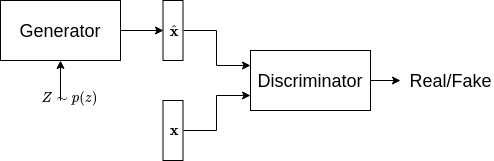
\includegraphics[scale=0.6]{./Figures/gan.png}
    \caption{High level architecture of Generative Adversarial Network. Both generator and discriminator are neural networks. Generator is supposed to generate samples $\hat{\mathbf{x}}$ that appear as if they are drawn from $p_d(\mathbf{x})$ and discriminator has to classify samples as real or fake depending on whether they come from $p_d(\mathbf{x})$ or generator.}
    \label{fig:gan}
\end{figure}

\subsection{Generative Adversarial Networks}
A generative adversarial network consists of two modules which are called \textit{generator} (G) and \textit{discriminator} (D). The generator takes a noise vector $\mathbf{z}$ as input and produces an output $\hat{\mathbf{x}}$ that is supposed to behave as a sample from the target distribution. The discriminator is trained to perform a binary classification task - that of classifying each sample as a real sample or a sample generated by the generator. This setup is depicted in Fig.~\ref{fig:gan}.

The generator and discriminators are trained alternatively. The objective of generator is to be able to fool the discriminator. Since the discriminator gets better over time, it forces the generator to become more clever which in turns challenges the abilities of discriminator and encourages it to get better. Note that in Fig.~\ref{fig:gan}, $\hat{\mathbf{x}} = G(\mathbf{z})$ where $\mathbf{z} \sim p(\mathbf{z})$. Usually $p(\mathbf{z})$ is a factored uniform noise distribution. In the same figure, $\mathbf{x}$ being fed to the discriminator is a randomly sampled training example. One can view this as a two player min-max game where the objective is as follows:
$$\min_G \max_D \mathbb{E}_{\mathbf{x} \sim p_d}[D(\mathbf{x})] - \mathbb{E}_{\mathbf{z} \sim p(\mathbf{z})}[D(G(\mathbf{z}))].$$

Although a GAN can be trained for generating samples from $p_d(\mathbf{x})$ directly, in what follows, the same idea will be used in a slightly different manner. The generator will be used to parameterize a proposal distribution so that MCMC framework can be used. This allows the method to inherit the nice properties of MCMC methods while still retaining expressive power of a neural network to learn an efficient proposal distribution.

\section{Markov Generative Adversarial Network (MGAN)}
Recall that we need to model the proposal distribution $q_\theta(. | x_t)$. Let $\pi_\theta^t$ denote the marginal distribution at time $t$, then two conditions must approximately hold:
\begin{enumerate}
    \item Suppose $\mathbf{x}_0 \sim \pi^0$ and let $\mathbf{x}_t \sim \pi_\theta^t$ after running a Markov chain with transition kernel given by $q_\theta(.|\mathbf{x}_t)$ for $t$ steps, then $\mathbf{x}_t$ must be close to samples obtained from $p_d$ for sufficiently large $t$.
    \item If $\mathbf{x}_0 \sim p_d$ and $\mathbf{x}_t$ is obtained as in the first point above, then $\mathbf{x}_t$ must be close to samples obtained from $p_d$ for sufficiently large $t$.
\end{enumerate}

Intuitively, the first condition suggests that $p_d$ should be the stationary distribution for Markov chain with transition kernel given by $q_\theta$. The second condition enforces that $p_d$ must be a fixed point for $q_\theta$. Markov GAN combines the two conditions together into a single objective function which is given by:
$$\min_G \max_D \mathbb{E}_{\mathbf{x} \sim p_d}[D(\mathbf{x})] - \lambda\mathbb{E}_{\bar{\mathbf{x}} \sim \pi_\theta^b}[D(\bar{\mathbf{x}})]  - (1 - \lambda) \mathbb{E}_{\mathbf{x}_d \sim p_d, \bar{\mathbf{x}} \sim T_\theta^m(\bar{\mathbf{x}} | \mathbf{x}_d)}[D(\bar{\mathbf{x}})].$$

Here $T_\theta^m(. | \mathbf{x})$ denotes the distribution over states of Markov chain after $m$ steps have been executed given that the Markov chain started in state $\mathbf{x}$ and $\lambda \in (0, 1)$ is a hyperparameter. The only issue now is to generate $\bar{\mathbf{x}}$ in a differentiable way so that standard gradient descent can be used. To achieve this, reparameterization trick is used. A sample $\mathbf{x}_{t + 1}$ from the distribution $q_\theta(. | \mathbf{x}_t)$ is modeled as:

$$\mathbf{x}_{t + 1} = f_\theta(\mathbf{x}_t, \mathbf{z}), \mathbf{z} \sim p(\mathbf{z}).$$

Here $f_\theta$ is a deterministic function that takes some random noise as input in the form of $\mathbf{z}$. Now the setup becomes end-to-end differentiable and it can be trained in the way a normal GAN is trained. The authors in \cite{SongEtAl:2017:ANiceMCAdversarialTrainingForMCMC} propose to sample $b \in [B]$ and $m \in [M]$ uniformly at random at each optimization step where $B$ and $M$ are hyperparameters to be set by the user and $[N] = \{1, 2, \dots, N\}$.


\section{Metropolis-Hasting based methods}

In the previous section, we considered sampling from a distribution whose analytical expression is unknown, but from which samples are available. Now, we consider the general problem of sampling from a continuous probability distribution $\pi(X), X \in \R^d$, whose analytical expression is known upto a multiplicative constant. These samples are then used for applications such as estimating $\E_{X \sim \pi} [f(X)]$ for some function $f$, etc. We wish to generate samples of $X$ as a Markov chain as $\{ X_t \}$. \\

Given a sample $X_t$ at step $t$, the next sample $X_{t+1}$ is generated by sampling a random variable $Y_{t+1}$ from a proposal distribution $q(.|X_t)$ and accepting $X_{t+1} = Y_{t+1}$ with acceptance probability

\EQ{
A(Y_{t+1} | X_t) = \min \lbrace 1, \frac{\pi(Y_{t+1})}{\pi(X_t)} \frac{q(X_t | Y_{t+1})}{q(Y_{t+1} | X_t)} \rbrace.
}

Rejecting $Y_{t+1}$ leads to setting $X_{t+1} = X_t$.\\

In the symmetric random walk setting, given sample $X_t$ at step $t$, we use the following transformation to obtain a proposed sample $Y_{t+1}$ for the next step.
\EQ{
Y_{t+1} = X_t + Z_t,
}
where $Z_t$ is a normal random variable, with mean $0$ and variance $\sigma^2 I_d$.

\subsection{Choice of $\sigma$}
The optimal choice of $\sigma$ is known only for very restrictive conditions on the distribution $\pi$. For example, if $\pi(x_1, x_2, .., x_d) = f(x_1).f(x_2) \dots f(x_d)$ or of the form $\pi(x_1, x_2, \dots, x_d) = \prod C_i f(C_i x_i)$, then the optimal value of $\sigma$ may be found analytically using $f$ and $C_i's$\cite{Rosenthal10optimalproposal}. As a special case, if $\pi$ is a normal distribution $\cN(0,\Sigma)$, and the proposal distribution is $\cN(0,\Sigma_p)$, then the optimal choice of $\Sigma_p$ is known to be $[ (2.38)^2 / D ] \Sigma$ to achieve an optimal acceptance rate of $2.38$. This optimal acceptance rate of $2.38$ also holds for slightly more general conditions in which the components of $\pi$ are independent, but each individual component is dominated by the sum of the components.

\subsection{Adaptive algorithms}
It is clear that since the above results hold under very special conditions, they are not guaranteed to work in most practical situations. However, they can be used as a heuristic to improve the performance of algorithms even in other situations. This can be done by hand using trial and error. For example, various values of variance of the proposal distribution or even various forms of the covariance matrix can be tried out and modified in such a way that the acceptance ratio is close to $0.238$.\\

However, this method is time consuming and also does not show much promise in improving the algorithm since choosing entries of a covariance matrix is a high dimensional problem and it would be unlikely that the we hit upon an optimal choice by trial and error.\\

To overcome this problem, algorithms have been proposed which automate the update of the parameters of the proposal distribution as the Markov chain progresses in time. Such algorithms are called adaptive algorithms \cite{Rosenthal10optimalproposal}.\\

For example, since it is known that if $\pi$ is a normal distribution $\cN(0,\Sigma)$, the optimal proposal distribution is the normal distribution with covariance matrix given by $(2.38)^2 / d$ times the target covariance matrix, the technique can be extended and used as a heuristic to obtain the following proposal distribution:

\EQ{
Y_{t+1} \sim \cN(X_t, [(2.38)^2/d] \Sigma_n),
}
where $\Sigma_n$ is the empirical covariance matrix of the first $t$ samples, which is used an estimate of the covariance matrix of the target distribution. This algorithm is called the Adaptive Metropolis algorithm.\\

Another approach is to use a mixture of two Gaussian distributions, one which is the same as above using the empirical covariance matrix and the other is a fixed Gaussian distribution for all time steps, i.e,

\EQ{
Y_{t+1} \sim (1 - \beta) \cN(X_t, [(2.38)^2/d] \Sigma_n) + \beta \cN(X_n, \Sigma_0)
}

\subsection{Metropolis adjusted Langevin algorithm}
The above approaches to designing the proposal distribution have not made use of information available in the form of $\pi$. In the above algorithms, the proposal random walk is the same irrespective of the current sample. One way to improve the algorithm to consider a proposal walk in the direction of increase of the probability density. One approach to this is the Metropolis adjusted Langevin algorithm which uses the following proposed increment distribution,

\EQ{
Z_{t+1} = \cN( \frac{\sigma^2}{2} \nabla \log \pi(X_t),\; \sigma^2 I_d ),
}
where $\nabla \log \pi(X_t)$ is the direction of steepest increase in $\log \pi(X_t)$. The value of $\sigma$ is chosen such that the acceptance rate is $0.574$, which has been proved to be optimal for the case of the components of the target distribution being independent and identically distributed.

\section{Hamiltonian Monte Carlo}
A drawback with the Metropolis adjusted Langevin algorithm is that at every point in the space, the proposed step is only towards the mode of the target distribution. But, especially in high dimensions, most of the probability mass of the distribution is located in a "typical set" which is far away from the mode and it is from this typical set from which we wish to sample most from \cite{2017arXiv170102434B}. \\

To use an analogy from physics, consider a system of a planet and a satellite. The planet produces a gravitational field and hence a potential energy analogous to $- \log \pi(X_t)$. A stationary satellite will collapse into the planet directly, which is what happens when using Langevin updates. But in the physical system, a suitable velocity given to the satellite will prevent its collapse and lets it stay in orbit around the planet, which is the typical set in our analogy. \\

For this purpose, along with the position $x$, we introduce an auxiliary random variable $v$, analogous to momentum/velocity. We wish to incorporate $v$ into the system such that the joint distribution of $(x,v)$ is given by

\EQ{
\pi_3(x,v) = \pi_2(v|x)\pi(x).
}

If the above holds, then sampling from the joint distribution of $(x,v)$ and ignoring the $v$ coordinate is equivalent to sampling $x$ from $\pi$.\\

Writing $\pi_3(x,v) = e^{-H(x,v)}$ so that $H(x,v)$ plays the role of energy of the system, we obtain

\EQ{
\begin{split}
H(x,v) &= - \log \pi_3(x,v) \\
	&= - \log \pi_2(v|x) - \log \pi(x) \\
	&= K(v,x) + U(x)  \text{  (say)}.
\end{split}
}

The function $U(x)$ plays the role of potential energy for the target distribution since $\pi(x) = e^{-U(x)}$ and $K(v,x)$ is analogous to kinetic energy of the particle.\\

Once we have the position and velocity of the particle, the next proposed state of the particle can be obtained using Hamilton's equations,

\EQ{
\begin{split}
\frac{dx}{dt} &= \frac{\partial H}{\partial v} = \frac{\partial K}{\partial v} \\
\frac{dv}{dt} &= - \frac{\partial H}{\partial x} = \frac{\partial K}{\partial x} - \frac{\partial U}{\partial x}.
\end{split}
}

where $\frac{dx}{dt}$ and $\frac{dv}{dt}$ are the rates of change of $x$ and $v$ respectively with respect to time $t$. The intuition for these equations is that a particle in a potential energy field moves in such a way that its total energy is conserved. This can be verified by seeing that $H(v,x)$ doesn't change with time.

\begin{align*}
\frac{dH(v,x)}{dt} &= \frac{\partial H}{\partial x} \frac{dx}{dt} + \frac{\partial H}{\partial v} \frac{dv}{dt} \\
	&= \frac{\partial H}{\partial x} \left( \frac{\partial H}{\partial v} \right) + \frac{\partial H}{\partial v} \left( - \frac{\partial H}{\partial x} \right) \\
	&= 0.
\end{align*}

So, given a state $(x,v)$, following the evolution of the state using the Hamilton's equations for some time gives the next proposed state. For that, we need to choose a form for the kinetic energy function. The most straightforward choice is $K(v,x) = \frac{1}{2} ||v||^2$, which leads to the distribution of $v$ to be 

\EQ{
\pi_2(v|x) = \frac{1}{(2\pi)^{\frac{d}{2}}} e^{-||v||^2/2}.
}

The normalizing constant for $\pi_2$ results in a constant being added to $K(v,x) = - \log \pi_2(v)$, which can be ignored since the evolution of the state with time depends only on the derivatives of the energy functions. \\

One way to move along the trajectory specified by the differential equations is called the leap frog integrator. In this method, for each time step, the value of $v$ is updated for half a time step, $x$ is updated for one time step and then $v$ is updated again for half a time step. These operations are repeated for $M$ time steps, for one  Hamiltonian Monte Carlo (HMC) transition.

\EQ{
\begin{split}
v^{\frac{1}{2}} &= v + \frac{\epsilon}{2} \frac{dv}{dt} = v - \frac{\epsilon}{2} \frac{\partial U}{\partial x} \\
x' &= x + \epsilon \frac{dx}{dt} = x + \epsilon v^{\frac{1}{2}} \\
v' &= v^{\frac{1}{2}} + \frac{\epsilon}{2} \frac{dv}{dt} = v^{\frac{1}{2}} - \frac{\epsilon}{2} \frac{\partial U}{\partial x}
\end{split}
}

It can be seen from the above set of equations that after applying them for one step, if the velocity variable is reversed and the transformations are applied for one time step, then we end up at the initial position and the negative of the initial velocity.

\begin{align*}
v'^{\frac{1}{2}} &= -v' - \frac{\epsilon}{2} \frac{\partial U}{\partial x} = - \left( v^{\frac{1}{2}} - \frac{\epsilon}{2} \frac{\partial U}{\partial x} \right) - \frac{\epsilon}{2} \frac{\partial U}{\partial x} \\
	&= - v^{\frac{1}{2}} \\
x'' &= x' + \epsilon v'^{\frac{1}{2}} = x' - \epsilon v^{\frac{1}{2}} \\
	&= x \\
v'' &= v'^{\frac{1}{2}} - \frac{\epsilon}{2} \frac{\partial U}{\partial x} = - v^{\frac{1}{2}} - \frac{\epsilon}{2} \frac{\partial U}{\partial x} \\
	&= - v.
\end{align*}

In other words, if we consider the transformation for obtaining the proposed next state as the composition of $M$ leap frog steps and a flip of the velocity vector, then the proposal distribution becomes symmetric. Let $f$ denote the transformation. Then, the Metropolis acceptance rate $A(\xi' | \xi)$ for a transition from state $\xi = (x,v)$ to $\xi' = (x',v')$ is given by

\EQ{
A(\xi' | \xi) = \min \{ 1, \frac{\pi(\xi')}{\pi(\xi)} \left| \frac{\partial f(\xi)}{\partial \xi} \right| \},
}

where $\left| \frac{\partial f(\xi)}{\partial \xi} \right|$ is the Jacobian of the transformation. In this case, the Jacobian turns out to be $1$, since the change of the set of variables which are being updated in each step of the transformation here depends only on the other variables which are unchanged in that step.

\section{Generalization of HMC}
The HMC algorithm has some obvious drawbacks. For example, if the distribution is multi modal, the algorithm may struggle to jump from one mode to another. This is due to the fact that the region between the modes may be of very low probability density and the velocity given to the particle may not be enough to jump over these regions which correspond to high potential energy. \\

One way to overcome this problem is to incorporate, in the transformation at each step, state dependent terms corresponding to scaling and translation\cite{levy2018generalizing}. These terms may be parameterized functions of the state and can be learnt by a gradient based algorithm. \\

Another further generalization has been proposed by Levy et al.\cite{levy2018generalizing}, along with the above idea. The update step of $x$ is further divided into two update steps. In the first step, half of the coordinates of $x$ are randomly chosen and updated and in the next step, the other half of the coordinates are updated. \\

However, in the process of generalization, care has to be taken so that the Jacobian of the transformation is tractable and can be easily calculable. A sufficient condition for this is to make sure when a set of variables are being affected in a step, their change depends only on other variables and not on any variable which is being updated. The transformation should also be invertible like the original HMC transformation. A proposed generalization satisfying these conditions is described below. \\

Consider the state space $\R^n$ on which the target distribution $\pi$ is defined. Let $x \in \R^n$ be a state. It is augmented by two additional random variables, $v \in \R^n$ representing velocity, which is sampled from a standard multivariate normal distribution and $d \in \{-1, 1\}$ which represents direction and is uniformly assigned one of its two possible values. Let the augmented state be denoted by $\xi \triangleq (x,v,d)$.

\subsection{Modified Leapfrog}
The modified leap frog operation consists of $M$ steps. At each step $t \in \{1, \dots, M \}$, a random mask $m^t \in \{ 0, 1 \}^n$ is sampled, which determines which coordinates of $x$ are transformed in the second step of the transformation and which are affected in the third. $m^t$ is drawn uniformly from the set of n-length binary vectors satisfying $ \sum_{i=1}^{n} m_i^t = \lfloor \frac{n}{2} \rfloor $. The coordinates of $x$ corresponding to ones in $m^t$ are updated first and the others next. Let $\bar{m}^t = \mathbb{1} - m^t$, where $\mathbb{1}$ is the n-dimensional vector of ones and let $x_{m^t} = x \odot m^t$, where $\odot$ represents element-wise multiplication. The following procedure is used to obtain the next state if $d=1$.\\

At each step of the transformation, an update to a set of variables depends only on the other variables. So, for the first step, in which $v$ is updated, let $\zeta_1 = (x, \partial_x U(x), t)$ be the tuple of the other variables, where $\partial_x U(x) = \frac{\partial U(x)}{\partial x}$. Then, the update of $v$ is given by

\EQ{
v' = v \odot \exp \left( \frac{\epsilon}{2} S_v(\zeta_1) \right) - \frac{\epsilon}{2} \left[ \partial_x U(x) \odot \exp \left( \epsilon Q_v(\zeta_1) \right) + T_v(\zeta_1) \right].
}

This is the same as the original leapfrog update, except that both $v$ and the gradient are scaled and a translation is applied to the scaled gradient. The functions $S_v, Q_v$ and $T_v$ used for the scaling and translation are parameterized by some parameter $\theta$ and are implemented by neural networks. If they are all identically zero, then we recover the standard leapfrog update. From the form of the transformation, it is clear that its Jacobian is $\exp(\mathbb{1}.S_v(\zeta_1))$. \\

Now, a modification similar to the one above is also made to the second update of the leapfrog operator after splitting it into two separate updates. Let $\zeta_2 \triangleq (x_{\bar{m}^t}, v, t)$ and $\zeta_3  \triangleq (x'_{m^t}, v, t)$.

\EQ{
\begin{split}
x' &= x_{\bar{m}^t} + m^t \odot \left[ x \odot \exp (\epsilon S_x(\zeta_2)) + \epsilon \left( v' \odot \exp(\epsilon Q_x(\zeta_2)) + T_x(\zeta_2) \right) \right], \\
x'' &= x'_{m^t} + \bar{m}^t \odot \left[ x' \odot \exp (\epsilon S_x(\zeta_3)) + \epsilon \left( v' \odot \exp(\epsilon Q_x(\zeta_3)) + T_x(\zeta_3) \right) \right].
\end{split}
}

The first equation affects only those coordinates of $x$ corresponding to ones in $m^t$ and hence the coordinates corresponding to $\bar{m}^t$ are fed to the scaling and translation functions and it is the other way around for the second equation. It is to be noted that these functions $S_x, Q_x$ and $T_x$ are different to those used in the update to $v$. The Jacobians for these transformations are $\exp(\epsilon m^t.S_x(\zeta_2))$ and $\exp(\epsilon \bar{m}^t.S_x(\zeta_3))$. \\

Now that $x$ is updated for one time step, finally, $v$ is updated for another half time step just as before. Let $\zeta_4 \triangleq (x'', \partial_x U(x''), t)$. Then,

\EQ{
v'' = v' \odot \exp \left( \frac{\epsilon}{2} S_v(\zeta_4) \right) - \frac{\epsilon}{2} \left[ \partial_x U(x'') \odot \exp(\epsilon Q_v(\zeta_4)) + T_v(\zeta_4) \right].
}

The Jacobian for this step is $\exp(\frac{\epsilon}{2} \mathbb{1}.S_v(\zeta_4))$. Let $L_\theta$ denote the composition of all these transformations applied one after the other for $M$ time steps. Let $F$ be the transformation of flipping the sign of $d$. Then, we obtain the Jacobian of the transformation as

\EQ{
\log \left| \frac{\partial [FL_\theta \xi]}{\partial \xi^T} \right| = d \sum_{t=1}^M \left[ \frac{\epsilon}{2} \mathbb{1}.S_v(\zeta_1^t) + \epsilon m^t.S_x(\zeta_2^t) + \epsilon \bar{m}^t.S_x(\zeta_3^t) + \frac{\epsilon}{2} \mathbb{1}.S_v(\zeta_4^t) \right]
}

Now, the above transformations are for the case $d=1$. For the case $d=-1$, we consider the opposite direction. So, we need to invert each of the above equations to obtain the required equations. Let $\zeta_1 \triangleq (x, \partial_x U(x), t)$. Then,

\EQ{
v' = \left[ v + \frac{\epsilon}{2} \left( \partial_x U(x) \odot \exp(\epsilon Q_v(\zeta_1)) + T_v(\zeta_1) \right) \right] \odot \exp(-S_v(\zeta_1)).
}

Let $\zeta_2 \triangleq (x_{m^t}, v, t)$. The second update can be written as

\EQ{
x' = x_{m^t} + \bar{m}^t \left[ x - \epsilon \left( v' \odot \exp(\epsilon Q_x(\zeta_2)) + T_x(\zeta_2) \right) \right] \odot \exp (- \epsilon S_v(\zeta_2)).
}

Letting $\zeta_3 \triangleq (x'_{\bar{m}^t}, v, t)$, the other coordinates of the position are updated as

\EQ{
x'' = x_{\bar{m}^t} + m^t \left[ x' - \epsilon \left( v' \odot \exp(\epsilon Q_x(\zeta_3)) + T_x(\zeta_3) \right) \right] \odot \exp (- \epsilon S_v(\zeta_3)).
}

Finally, letting $\zeta_4 \triangleq (x'', \partial_x U(x''), t)$, the velocity is updated as

\EQ{
v' = \left[ v + \frac{\epsilon}{2} \left( \partial_x U(x) \odot \exp(\epsilon Q_v(\zeta_4)) + T_v(\zeta_4) \right) \right] \odot \exp(-S_v(\zeta_4)).
}

The above transformations are applied consecutively for $M$ time steps for $t=M,M-1, \dots, 1$ to obtain a transformation denoted by $L_\theta$ and then a flip transformation $F$ is applied which flips the direction/sign of $d$. The Jacobian can similarly be obtained as before. \\

From the way the transformations are defined, it is easy to see that with $L_\theta \xi = L\theta(x,v,d) = (x''^{\times M}, v''^{\times M}, d)$ and $F \xi = (x, v, -d)$, $FLFL(x,v,d) = (x,v,d)$. Since the distribution of $v$ is symmetric and the transformation is invertible with its inverse being itself, the transition kernel is symmetric. So, the metropolis acceptance probability becomes

\EQ{
A(FL \xi | \xi) = \min \left( 1, \frac{p(FL \xi)}{p(\xi)} \left| \frac{\partial [FL \xi]}{\partial \xi^T} \right| \right),
}

where $p(\xi) = \pi(x) \pi_v(v) \pi_d(d)$, $\pi(x)$ is the target distribution, $\pi_v$ is the standard multivariate normal distribution and $p_d$ is a uniform distribution over $\{-1, 1\}$. \\

For notational simplicity, consider the step of resampling momentum and direction at each step as the operator $R$, i.e, $R(x,v,d) = (x, v', d')$, where $v' \sim \cN(0, I_n)$ and $d \sim \mathcal{U}(\{ -1, 1 \})$. \\

Using this notation, the Markov chain can be described as a repeated loop of the following steps:

\begin{enumerate}
\item $\xi' = FL_\theta \xi$ with probability $A(FL_\theta \xi | \xi)$, otherwise $\xi' = \xi$.
\item $\xi = R \xi'$.
\end{enumerate}

Each $Q,S$ and $T$ is a neural network with two hidden layers of $100$ units each and ReLU non-linearities and the output layer has a tanh activation. The time step $t$ is given as input to the networks as $\tau(t) = ( \cos(\frac{2 \pi T}{M}), \sin(\frac{2 \pi T}{M}) )$. \\

\subsection{Loss}
To find the optimal parameters for the functions described above, we need a suitable objective function with respect to which they can be optimized. One option is to minimize lag one correlation, which is equivalent to maximizing the expected square jump distance. Let $\delta (\xi', \xi) = \delta ( (x', v', d'), (x, v, d) ) = ||x' - x||^2$ be the squared distance. Then, we wish to maximize the expected square distance $\E_{\xi \sim p(\xi)} [\delta(FL_\theta \xi, \xi) A(FL_\theta \xi | \xi)]$. But, this is an average over the entire space. This means that even if this is optimized, there may be regions in the space where this may be too low. To avoid this situation, we define the following loss function to be minimized:

\EQ{
l_\lambda(\xi, \xi', A(\xi' | \xi)) = \frac{\lambda^2}{\delta(\xi, \xi') A(\xi' | \xi)} - \frac{\delta(\xi, \xi') A(\xi' | \xi)}{\lambda^2}.
}

The second term encourages typical moves to be large on average and the first term highly penalizes any situation in which the jump distance or the acceptance probability is very low. We wish to minimize this loss averaged over the target distribution to encourage mixing of the Markov chain when it is close to the target distribution. Other than that, we also wish to make the chain burn in fast, i.e, it should explore the space efficiently even when it is close to the initial distribution. So, considering the initial distribution to be $q(\xi) = \pi_0(x) \pi_v(v) \pi_d(d)$, the objective is to minimize the loss

\EQ{
\sL(\theta) \triangleq \E_{p(\xi)}[l_\lambda(\xi, FL_\theta \xi, A(FL_\theta \xi | \xi))] + \lambda_b \E_{q(\xi)}[l_\lambda(\xi, FL_\theta \xi, A(FL_\theta \xi | \xi))].
}

The first term encourages mixing and the second term encourages fast burn-in and $\lambda_b$ determines how much importance we wish to give to burn-in.

\subsection{Optimization}
Now that we have an objective function, we can tune the parameters to optimize it. The expectation in the loss is estimated by sampling from the corresponding distributions. $q(\xi)$ is chosen such that it can easily be sampled from. The expectation over $p(\xi)$ is estimated using samples from the Markov chain itself and the loss is calculated for each sample. \\
A batch of $N$ samples is used for calculating the total loss. From that, we may calculate gradient of the loss with respect to the parameters of the neural networks, which is used for updating the parameters in a gradient based algorithm, with some time dependent learning rate $\alpha_t$. The algorithm can be written as follows:

\begin{algorithm}
\caption{Training the Markov chain}\label{Training}
\begin{algorithmic}[0]


\State Initialize $\theta$
\State Initialize $\{ \xi_p^{(i)} \}_{1 \leq i \leq N}$ from $q(\xi)$
\For{$t$ from $0$ to $n_{iters} - 1$}
	\State Sample a mini batch $\{ \xi_q^{(i)} \}_{1 \leq i \leq n}$ from $q(\xi)$
	\State $L \leftarrow 0$
	\For{$i$ from $1$ to $N$}
		\State $\xi_p^{(i)} \leftarrow R \xi_p^{(i)}$
		\State $L \leftarrow L + l_\lambda(\xi_p^{(i)}, FL_\theta \xi_p^{(i)}, A(FL_\theta \xi_p^{(i)} | \xi_p^{(i)})) + \lambda_b l_\lambda(\xi_q^{(i)}, FL_\theta \xi_q^{(i)}, A(FL_\theta \xi_q^{(i)} | \xi_q^{(i)}))$
		\State $\xi_p^{(i)} \leftarrow FL_\theta \xi_p^{(i)}$ with probability $A(FL_\theta \xi_p^{(i)} | \xi_p^{(i)})$
	\EndFor
	\State $\theta \leftarrow \theta - \alpha_t \nabla_\theta L$
\EndFor

\end{algorithmic}
\end{algorithm}

\clearpage

\bibliographystyle{unsrt}
\bibliography{\jobname}


\end{document}
